\documentclass{article}

\usepackage{full page}
\usepackage{pdfpages}
\usepackage{graphicx}
\usepackage{float}
\usepackage{mdframed}
\usepackage{minted}
\usepackage{enumerate}


\usepackage{listings}
\lstset{language=Python}

\title{Profile Hidden Markov Models}
\author{Taylor Cathcart, Cam Setian, Kyle Tessier-Lavigne}

\begin{document}
\maketitle

\section{Introduction}
As the cost of genetic sequencing has dropped significantly over the past decade, there has become an abundance of unprocessed genetic data. Many different computational methods have been developed or adapted to look for patterns in sets of genetic sequences, including Hidden Markov Models, which are particularly useful for processing signals from noise. One of the first applications of HMMs was in speech recognition in the 70s, and since then, many uses have been found in biological sequence analysis, including gene prediction, sequence alignment, structural alignment, and more.\footnotemark[1] In this paper, we use profile-HMMs to *** need to figure out what we're doing with them ***


\footnotetext[1]{Hidden Markov Models and their Applications in Biological Sequence Analysis. Current Genomics. Sep 2009; 10(6): 402-415}


\section{Methods}

\subsection{Hidden Markov Models}
A Hidden Markov Model describes the probabilistic relationship between a set of hidden (i.e. unobservable) states and a set of known observations. If one knows the probability of going from one state to another at each time interval (the transition probability), and the probability that a given observation will be expressed by each state (the emission probability), then given a sequence of observations, one should be able to use this model to predict the most likely sequence of states corresponding to those observations. For example, say two people, Ann and Bob, live far apart. Bob tells Ann what he did each day for a week. Ann, who lives far from Bob, doesn't know what the weather is like for Bob each day. However, Ann does know the probability that Bob will do a certain activity based on the weather where he lives. She also knows the probability that a rainy day will be followed by a sunny day, and vice-versa. Using this information (where the weather reprsents the unobservable state, and the activity represents the observation for that day), Ann should be able to figure out the most likely weather pattern for that week.
\begin{figure}[H]
\centering
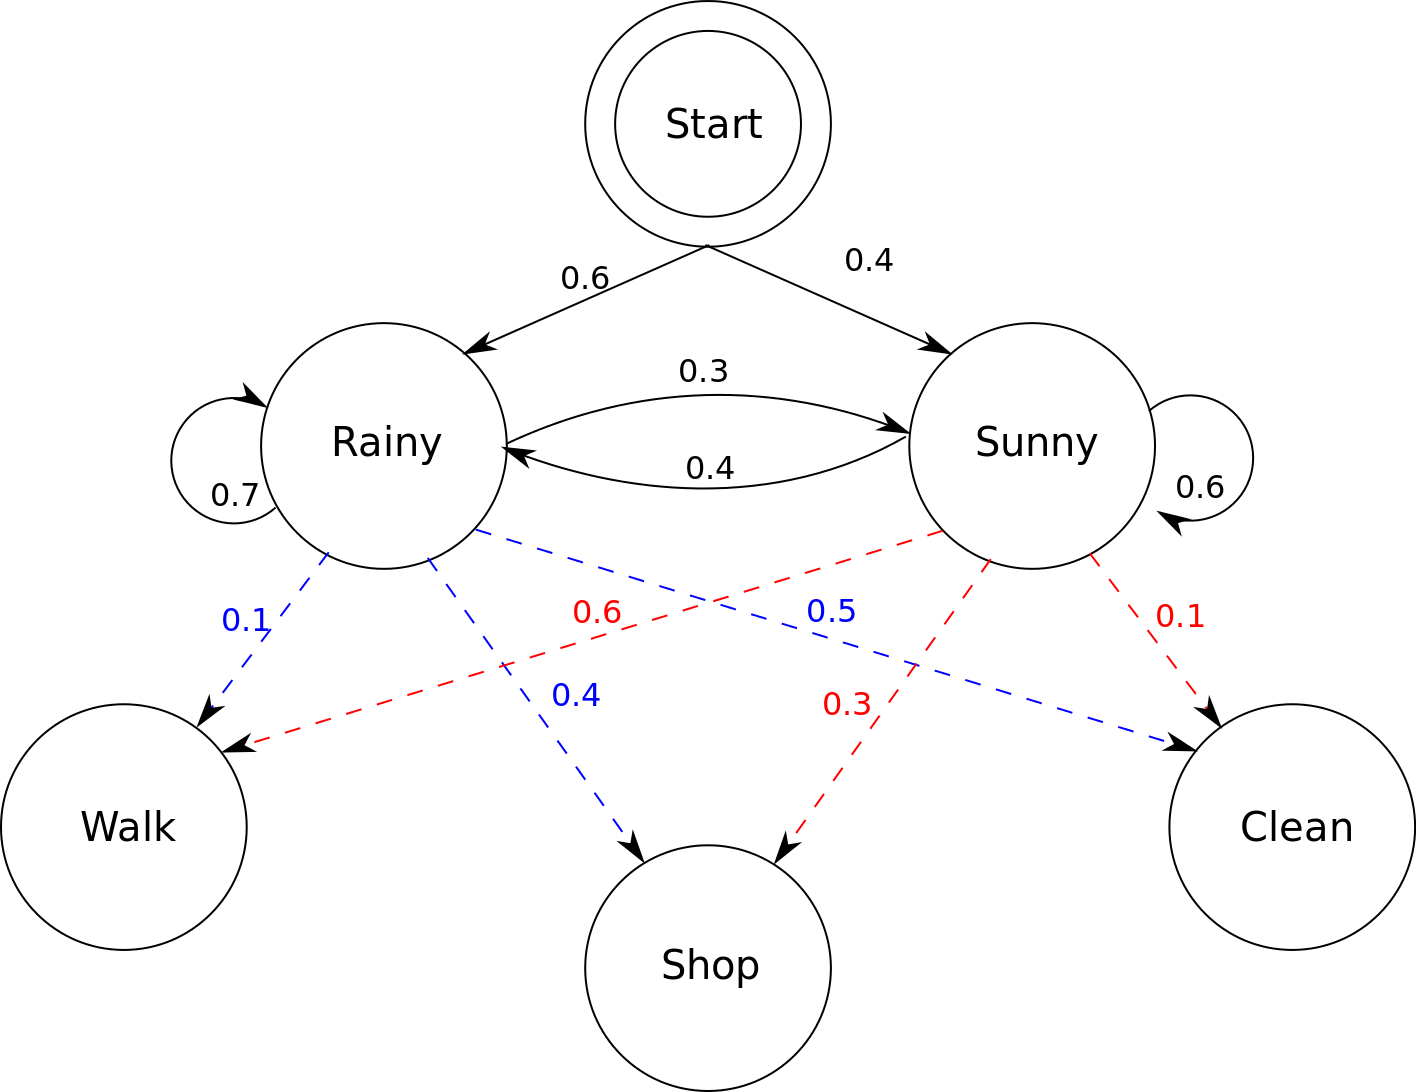
\includegraphics[width=.5\textwidth]{materials/HMMGraph.png}
\caption{Transition probabilities between states, and their emission probabilities for each observation\footnotemark[2]}
\end{figure}

\footnotetext[2]{http://en.wikipedia.org/wiki/File:HMMGraph.svg}

\subsection{Profile-Hidden Markov Models}
Profile-Hidden Markov Models are an adaptation of HMMs used to model genetic sequences. A profile-HMM consists of a sequence of match, insert, and delete states which span the length of the consensus sequence. A match corresponds to the expression of either a nucleotide (in the case of DNA sequencing) or an amino acid (in the case of protein sequencing). Insert and delete states correspond to the expression of a gap. 

\subsection{Viterbi Training}

\subsection{Baum-Welch Training}


\section{Applications}

\section{Results}

\section{Discussion}


% Example for formatting code:
% 
% \begin{minted}[mathescape, linenos, numbersep=3pt, gobble=0, framesep=20mm]{python}
% 
% if __name__ == '__main__':
% 	print 'hello world'
% 
% \end{minted}



% Example for inserting figures:
% 
% \begin{figure}[H]
% \centering
% \includegraphics[width=.5\textwidth]{filename goes here}
% \caption{\bf caption goes here}
% \end{figure}


\end{document}